%\documentclass[german,10pt]{book}      
\usepackage{makeidx}
\usepackage{babel}            % Sprachunterstuetzung
\usepackage{amsmath}          % AMS "Grundpaket"
\usepackage{amssymb,amsfonts,amsthm,amscd} 
\usepackage{mathrsfs}
\usepackage{rotating}
\usepackage{sidecap}
\usepackage{graphicx}
\usepackage{color}
\usepackage{fancybox}
\usepackage{tikz}
\usetikzlibrary{arrows,snakes,backgrounds}
\usepackage{hyperref}
\hypersetup{colorlinks=true,
                    linkcolor=blue,
                    filecolor=magenta,
                    urlcolor=cyan,
                    pdftitle={Overleaf Example},
                    pdfpagemode=FullScreen,}
%\newcommand{\hyperref}[1]{\ref{#1}}
%
\definecolor{Gray}{gray}{0.80}
\DeclareMathSymbol{,}{\mathord}{letters}{"3B}
%
\newcounter{num}
\renewcommand{\thenum}{\arabic{num}}
\newenvironment{anmerkungen}
   {\begin{list}{(\thenum)}{%
   \usecounter{num}%
   \leftmargin0pt
   \itemindent5pt
   \topsep0pt
   \labelwidth0pt}%
   }{\end{list}}
%
\renewcommand{\arraystretch}{1.15}                % in Formeln und Tabellen   
\renewcommand{\baselinestretch}{1.15}                 % 1.15 facher
                                                      % Zeilenabst.
\newcommand{\Anmerkung}[1]{{\begin{footnotesize}#1 \end{footnotesize}}\\[0.2cm]}
\newcommand{\comment}[1]{}
\setlength{\parindent}{0em}           % Nicht einruecken am Anfang der Zeile 

\setlength{\textwidth}{15.4cm}
\setlength{\textheight}{23.0cm}
\setlength{\oddsidemargin}{1.0mm} 
\setlength{\evensidemargin}{-6.5mm}
\setlength{\topmargin}{-10mm} 
\setlength{\headheight}{0mm}
\newcommand{\identity}{{\bf 1}}
%
\newcommand{\vs}{\vspace{0.3cm}}
\newcommand{\noi}{\noindent}
\newcommand{\leer}{}

\newcommand{\engl}[1]{[\textit{#1}]}
\parindent 1.2cm
\sloppy

         \begin{document}  \setcounter{chapter}{5}

\chapter{EPR -- Bell -- CHSH}
% Kap x
\label{chap_EPR}


\info{Thomas Filk}{31.03.2024}%
Im Jahre 1935\index{Einstein, Albert} 
ver\"offentlichten Albert Einstein,
Boris Podolsky\index{Podolsky, Boris}\index{Rosen, Nathan} 
und\index{Einstein-Podolsky-Rosen (EPR)} 
Nathan Rosen einen Artikel 
{\em Can quantum-mechanical description of physical
reality be considered complete?} \cite{EPR} Dieser Artikel machte
die ungew\"ohnlichen und \"uberraschenden
Folgerungen aus der Existenz
verschr\"ankter Zu\-st\"ande in der Quantentheorie
besonders deutlich und er ist immer noch
Gegenstand von Grundsatzdiskussionen zur
Quantentheorie. Der Angriff der drei Autoren -- kurz EPR genannt --
galt der Behauptung, die Quantenmechanik sei
vollst\"andig und w\"urde 
allen Freiheitsgraden Rechnung tragen, die
physikalisch von Bedeutung und sinnvoll sind. 
In ihrer Arbeit kamen sie zu dem Schluss, 
dass es gewisse\index{Elemente der Realit\"at} 
\glqq Elemente der Realit\"at\grqq\ geben
m\"usse, die von der Quantenmechanik nicht
beschrieben werden. Daher sei diese nicht
vollst\"andig.

John Bell griff 1964 die Ideen von EPR auf und entwickelte 
Kriteria, wie man entscheiden k\"onne, ob es diese Elemente der
Realit\"at wirklich gibt \cite{Bell4}. Diese Kriterien wurde von John F.\ Clauser et al.\
weiterentwickelt zu den sogenannten CHSH-Ungleichungen \cite{CHSH}, deren
Verletzung in der Quantentheorie 1982 durch Alain Aspect 
zweifelsfrei nachgewiesen werden konnte \cite{Aspect}. Die notwendige
Schlussfolgerung aus diesen Experimenten ist, dass die Quantentheorie
in einem gewissen Sinn eine nicht-lokale Theorie ist.  

\section{EPR und Quantenkorrelationen}
\label{sec_EPR}

EPR haben urspr\"unglich ihr scheinbares Paradoxon
anhand eines Zweiteilchensystems beschrieben, bei dem die
Orts- und Impulsvariablen der einzelnen Teilchen 
verschr\"ankt sind. Das Zwei\-teilchen\-sys\-tem wird durch einen Zustand
beschrieben, bei dem der Gesamtimpuls $\pmb{P}_1+\pmb{P}_2$
und die Relativkoordinate $\pmb{Q}_1-\pmb{Q}_2$ festliegen. Dies ist kein Widerspruch, da diese
beiden Gr\"o\ss en miteinander kommutieren. Ich beschreibe hier
das Paradoxon anhand der Spinfreiheitsgrade von zwei
Elektronen. Diese Version geht auf\index{Bohm, David} 
David Bohm zur\"uck
und vermeidet die formalen Schwierigkeiten im Zusammenhang
mit den Eigenfunktionen zum Ort bzw.\ Impuls, die nichts mit
dem eigentlichen Problem zu tun haben. Statt
der Spinfreiheitsgrade kann man ebenso gut
auch die Polarisationsfreiheitsgrade von Photonen
betrachten.

\subsection{Der EPR-Zustand}

Gegeben seien zwei Spin-$\frac{1}{2}$-Teilchen in dem
Zustand, bei dem der Gesamt\-drehimpuls $S=S_1+S_2$
verschwindet.
Der Vektor zu diesem sogenannten\index{EPR-Zustand} 
EPR-Zustand hat die Form:
\begin{equation}
\label{eq_Multi_EPR}
      |\Psi_{\rm EPR}\rangle = \frac{1}{\sqrt{2}} \left(
        | \uparrow \rangle_1 \otimes |\downarrow \rangle_2 -
        |\downarrow \rangle_1 \otimes |\uparrow \rangle_2 \right) 
\end{equation} 
Die Indizes 1 und 2 beziehen sich dabei auf Teilchen 1
und Teilchen 2. Diese beiden Teilchen k\"onnen unterscheidbar sein,
entweder, weil sie einen gro\ss en Abstand voneinander haben und
der Ort die Teilchen identifiziert,
oder weil es sich um verschiedene Teilchenarten handelt --
EPR setzen nicht voraus, dass die verschr\"ankten Sys\-teme
ununterscheidbar sind. Die Symbole $\uparrow$ und $\downarrow$ 
in den Ket-Klammern bezeichnen die beiden m\"oglichen
Polarisationen des Spins bez\"uglich einer vorgegebenen
Richtung, beispielsweise der $z$-Richtung. Allerdings ist
der Zustand invariant unter beliebigen Drehungen
(es handelt sich um den rotationssymmetrischen 
Zustand mit Gesamt\-dreh\-impuls $S=0$), die Antikorrelation gilt also 
bez\"uglich jeder Richtung \hyperref[sec_EPR_A]{(Herleitung 1)}. 

Dieser Zustandsvektor\index{verschr\"ankt} 
ist verschr\"ankt, d.h., es gibt keine Basis, in
der dieser Zustand faktorisiert. Keinem der beiden Teilchen
kann ein wohldefinierter Spinzustand zugesprochen werden.
Bildet man die Teilspur \"uber einen Spinfreiheitsgrad %  ((vorrechnen?))
erh\"alt man f\"ur den verbliebenen Freiheitsgrad 
$\rho=\frac{1}{2} \identity$, also
eine Dichte\-mat\-rix zu \glqq maximaler Unkenntnis\grqq. Durch
lokale Messungen, also Messungen an nur einem der
Spinfreiheitsgrade, kann man diesen Zustand nicht von einem
Gemisch von Spinzust\"anden unterscheiden \hyperref[sec_EPR_B]{(Herleitung 2)}. 

Der EPR-Zustand ist eine Superposition von zwei Beitr\"agen,
bei denen jeweils eine Spinkomponente eines Teilchens
antikorreliert ist mit der entsprechenden Spinkomponente 
des anderen Teilchens. Wann immer man an einem Teilchen
eine Messung des Spins bez\"uglich irgendeiner Richtung
vornimmt, wei\ss\ man, dass die Spinkomponente
des anderen Teilchens bez\"uglich derselben Richtung den
entgegengesetzten Wert hat. Diese Eigenschaft kann man
an beliebig vielen gleichartig pr\"aparierten Systemen
kontrollieren: Bez\"uglich derselben Richtung sind die
beiden Spinkomponenten immer antikorreliert! 

\subsection{Das EPR-Argument}

EPR argumentieren nun folgenderma\ss en: Wenn wir an
Teilchen 2 eine Spinmessung bez\"uglich irgendeiner 
Richtung vornehmen, k\"onnen wir das Ergebnis der 
entsprechenden Messung an dem anderen Teilchen mit 
100-prozentiger Sicherheit vorhersagen, ohne an diesem
Teilchen irgendeine Ver\"anderung (Messung) vorgenommen 
zu haben.\footnote{Hier hilft es, sich die beiden Teilchen in sehr
gro\ss er Entfernung voneinander vorzustellen.
Verschr\"ankte Zust\"ande wurden \"uber mehr als 1200\,km  Abstand
nachgewiesen \cite{Yin}. Im Prinzip setzt die Quantentheorie hier aber keine
Grenzen, sodass auch Messungen an Teilchenpaaren -- eines hier 
auf der Erde und das andere in einer anderen Galaxie --
diese Ergebnisse liefern sollten.} Da Teilchen 1 aber nicht \glqq wei\ss\grqq, 
bez\"uglich welcher Richtung an Teilchen 2 eine
Messung vorgenommen wird, wir aber trotzdem anschlie\ss end
vorhersagen k\"onnen, was eine Messung an diesem Teilchen
bez\"uglich der (von dem Experimentator willk\"urlich gew\"ahlten) Richtung 
ergeben wird, muss dieses Ergebnis schon vorher festliegen.
Es muss also einen bisher nicht bekannten Freiheitsgrad
geben, der f\"ur dieses Ergebnis verantwortlich ist. Diese
Forderung bezeichnen EPR als \glqq Elemente
der Realit\"at\grqq. Ihre Definition lautet: \glqq Wenn wir an
einem Sys\-tem, ohne dieses in irgendeiner Weise zu st\"oren,
mit Sicherheit ... das Ergebnis einer Messung vorhersagen
k\"onnen, dann muss es ein Element der Realit\"at geben,
das diesem Freiheitsgrad entspricht\grqq. Da die
Quantenmechanik diesem Element der Realit\"at nicht
Rechnung tr\"agt, ist die Quantenmechanik nicht
vollst\"andig.

Interessant ist, dass EPR in ihrem Artikel nicht
die Widerspruchsfreiheit des quantenmechanischen
Formalismus angreifen. Sie h\"atten dies durch folgende
Argumentation scheinbar leicht tun k\"on\-nen:
Angenommen, wir messen die Spinorientierung an Teilchen
2 in $x$-Richtung. Dann kennen wir damit auch die
Spinorientierung von Teilchen 1 in $x$-Richtung (wegen der
Antikorrelation). Messen wir nun die Spinorientierung von
Teilchen 1 in $z$-Richtung, kennen wir sowohl seine
Spinorientierung in $z$- als auch in $x$-Richtung, was nach
den Unsch\"arferelationen nicht m\"oglich sein sollte.
In \"ahnlicher Form hatte Einstein bei seinen fr\"uheren
Angriffen auf die Quantenmechanik argumentiert.
Bohr hatte immer damit gekontert, dass wir die
Vorhersage, die wir f\"ur die $x$-Richtung der Spinorientierung
von Teilchen 1 treffen, nicht mehr kontrollieren k\"onnen,
nachdem wir die $z$-Richtung gemessen haben.
Somit sei diese Vorhersage nicht \"uberpr\"ufbar.
EPR greifen in ihrem Artikel die scheinbare 
Unvollst\"andigkeit der Quantenmechanik an, nicht 
ihre scheinbare Widerspr\"uchlichkeit. Dieses Beispiel macht auch
nochmals deutlich, dass es bei dem quantenmechanischen Zustandsbegriff
nicht um unser scheinbares Wissen \"uber ein System geht, sondern
um die M\"oglichkeiten von \"uberpr\"ufbaren Vorhersagen.

Damit richtete sich die Kritik von EPR direkt gegen das Theorem von Neumanns.
Dieser hatte in seinem Buch bewiesen, dass man die Quantenmechanik
nicht um verborgene Variable erweitern kann, ohne die \"uberpr\"ufbaren Vorhersagen
der Quantenmechanik abzu\"andern. 
 
Es sollte abschlie\ss end noch betont werden, dass die
Korrelationen bzw.\ Antikorrelationen von verschr\"ankten
Zust\"anden nicht zu einer kontrollierten Signal\-\"uber\-tragung
(und damit zu einer Kommunikation) verwendet
werden k\"onnen, da man als Experimentatorin oder Experimentator 
keinen Einfluss auf das Ergebnis einer Spinmessung hat. In diesem Sinne gleichen diese
Korrelationen sogenannten Common-Cause-Korrelationen\index{Common-Cause-Korrelation}
in klassischen Systemen, bei
denen aufgrund einer gemeinsamen Ursache (dem Common Cause) eine
Korrelation vorliegt. Beispielsweise kann eine Person zwei
Briefe identischen Inhalts an zwei andere, weit voneinander
entfernte Personen schicken, die diese Briefe gleichzeitig
\"offnen und somit zeitgleich wissen, was die andere Person
in diesem Augenblick liest. Trotzdem kann die eine Person
der anderen Person auf diese Weise keine Information senden.
Es gibt in diesem Fall jedoch die
\glqq Elemente der Realit\"at\grqq, denn der Inhalt der
Briefe liegt ja schon vor, bevor die Personen die Briefe
\"offnen. Eine \"ahnliche \glqq verborgene Variable\grqq\
stellten sich wohl auch EPR vor, als sie das Paradoxon
formulierten und zu dem Schluss kamen, die Quantentheorie sei nicht
vollst\"andig. Wie wir in Abschnitt \ref{sec_Bell} sehen werden,
kann es verborgene Variable dieser Art in der Quantentheorie
nicht oder nur unter sehr eingeschr\"ankten Bedingungen geben.

\subsection{Zeitgen\"ossische Reaktionen auf EPR}

Die Reaktion der zeitgen\"ossischen Physiker und 
Mitbegr\"under der Quantenmechanik auf den Artikel von Einstein,
Podolsky und Rosen war sehr
unterschiedlich.\index{Pauli, Wolfgang} 
Wolfang Pauli schrieb unmittelbar nach der
Ver\"offentlichung einen Brief an Werner 
Heisenberg, in dem\index{Heisenberg, Werner}
er ihn aufforderte, eine Antwort auf den EPR-Artikel
zu verfassen \cite{Pauli}. In diesem Brief bemerkt er unter anderem:
\textit{Einstein hat sich wieder einmal zur Quantenmechanik
\"offentlich ge\"au\ss ert ... (gemeinsam mit Podolsky und Rosen --
keine gute Kompanie \"ubrigens). Bekanntlich ist das jedes
Mal eine Katastrophe, wenn es geschieht. \glq Weil, so schlie\ss t
er messerscharf - nicht sein kann, was nicht sein darf.\grq\ 
(Morgenstern). ... Immerhin m\"ochte ich ihm zugestehen,
dass ich, wenn mir ein Student in j\"ungeren Semestern
solche Einw\"ande machen w\"urde, diesen f\"ur ganz
intelligent und hoffnungsvoll halten w\"urde.} \cite{Pauli}

Die Argumentation von EPR 
ist verbl\"uffend einfach und dementsprechend
hatte beispielsweise\index{Bohr, Niels} 
Niels Bohr gro\ss e Schwierigkeiten, eine
passende Antwort zu finden. Sein damaliger Assistent L\'{e}on
Rosenfeld schreibt dazu \glqq ... this onslaught came down on
us as a bolt from the blue\grqq, und er beschreibt die
Schwierigkeiten, die Bohr bei der Formulierung der Antwort hatte.

In einem Artikel
mit demselben Titel wie die EPR-Arbeit \cite{Bohr2}
schreibt Niels Bohr, dass eine physikalische Messung (hier an Teilchen 2)
nicht unbedingt eine \glqq mechanische St\"orung\grqq\ f\"ur
Teilchen 1 bedeuten muss (wie schon erw\"ahnt, k\"onnen die beiden Teilchen
theoretisch Lichtjahre voneinander entfernt sein und die
jeweiligen Messungen innerhalb der jeweiligen Lichtkegel
-- also im Sinne der Relativit\"atstheorie au\ss erhalb der 
jeweiligen kausalen Einflussbereiche --
stattfinden). Er f\"ahrt dann aber fort, dass eine solche Messung
jedoch \glqq
einen Einfluss auf die M\"oglichkeiten der Vorhersagen
zuk\"unftiger Messungen\grqq\ hat. Die Antwort von Bohr
wird oftmals so gedeutet, dass er dem Quantenzustand
eines Systems keine von unserer Erfahrung unabh\"angige
Realit\"at zuschreibt und dieser somit subjektiv ist. Die
Reduktion besteht f\"ur Bohr (und Heisenberg hat dies
sp\"ater explizit betont \cite{Heisenb}) lediglich in der \"Anderung unseres
Wissens \"uber das System.

Der Begriff \glqq Verschr\"ankung\grqq\ wurde von Erwin Schr\"odinger 
gepr\"agt und erscheint zum ersten Mal
in einer Reihe von Artikeln, die man als Kommentare zur EPR-Arbeit
auffassen kann und die den damaligen Stand der naturwissenschaftlichen und
naturphilosophischen Erkenntnisse in Bezug auf die Quantentheorie
zusammenfassten \cite{Schroedinger}. Auch Schr\"odinger betont die
Subjektivit\"at des Quantenzustands, indem er \glqq die Wellenfunktion
als Katalog von Erwartungen\grqq\ beschreibt.      
 
\section{Bell'sche Ungleichungen}
\label{sec_Bell}

Mitte der 1960er Jahre ging John Bell\index{Bell, John} 
in mehreren Artikeln der Frage nach, ob es diese
\glqq Elemente der Realit\"at\grqq\ -- heute w\"urde
man meist von \glqq verborgenen Variablen\grqq\ sprechen,
da diese Freiheitsgrade nach der Quantentheorie nicht
beobachtbar sein sollten -- wirklich geben kann \cite{Bell3,Bell4}.
Zu diesem Zeitpunkt gab es bereits mehrere
sogenannte\index{verborgene Variable, No-Go-Theoreme} 
No-Go-Theoreme, welche die Existenz
verborgener Variabler auszuschlie\ss en schienen. 
Das bekannteste
dieser No-Go-Theoreme stammte von John von
Neumann\index{von Neumann, John!No-Go-Theorem} 
(damals nannte er sich noch Johann von Neumann)
und wurde 1932 in seinem Buch zu den mathematischen
Grundlagen der Quantenmechanik \cite{Neumann}
ver\"offentlicht. (Eine sehr fr\"uhe Kritik an diesem Theorem
kam von der Philosophin und Mathematikerin Grete Hermann.)   %  mehr Info zu Grete Hermann?

Nachdem David Bohm im Jahre 1952\index{Bohm, David} 
eine Erweiterung der Quantenmechanik im Sinne von verborgenen
Variablen gelang und somit das scheinbar Unm\"ogliche
wahr geworden war, machte sich John Bell an die
Untersuchung der bisherigen No-Go-Theoreme,
um deren Schwachstellen zu finden. Insbesondere
war ihm bewusst, dass die 
Bohm'sche Mechanik\index{Bohm'sche Mechanik}
keine lokale Theorie ist, d.h., physikalisch objektiv
vorhandene Entit\"aten (das F\"uhrungsfeld) \"andern
sich instantan und global als Folge einer Messung. 
Bells eigentliches Anliegen war die Frage, 
ob man nicht eine Theorie mit
verborgenen Variablen konstruieren kann, die
lokal, d.h., mit dem Kausalit\"atsverst\"andnis
der Relativit\"atstheorie vereinbar ist. Das Ergebnis
seiner \"Uberlegungen -- die Bell'schen 
Ungleichungen -- zeigen, dass keine lokale Theorie von 
verborgenen Variablen
die experimentellen Vorhersagen der Quantenmechanik
reproduzieren kann.

\subsection{Bell'sche Ungleichungen -- die Version von
Wigner und d'Espagnat}
\label{sec_Espagnat}

Die folgende anschauliche Herleitung einer 
Bell'schen Ungleichung (es gibt mehrere verschiedene
Versionen\index{Bell'sche Ungleichungen} 
von Bell'schen Ungleichungen) geht urspr\"unglich
auf Eugene Wigner\index{Wigner, Eugene P.} 
und in der hier vorgestellten Form
auf\index{Despagnat@d'Espagnat, Bernard} 
Bernard d'Espagnat zur\"uck \cite{Espagnat}.

Wir nehmen an, es gebe drei verschiedene Observablen
$A$, $B$ und $C$, die als Ergebnisse jeweils nur zwei
m\"ogliche Werte (z.B.\ $+1$ und $-1$) zulassen. Ein klassisches
Beispiel w\"are ein System aus drei M\"unzen, die
jeweils \glqq Kopf\grqq\ oder \glqq Zahl\grqq\ zeigen
k\"onnen. Aus einem tieferliegenden Grund (in der Quantentheorie
aufgrund nicht kommutierender Observablen) kann man aber
an einem System jeweils nur zwei dieser Observablen
messen, daf\"ur kann man aber an beliebig vielen
gleichartig pr\"aparierten Systemen solche
Messungen vornehmen. Wir teilen nun ein ausreichend
gro\ss es Ensemble solcher Systeme in drei gleich
gro\ss e Gruppen. Bei der ersten Gruppe messen
wir die Observablen $A$, $B$, bei der zweiten die
Observablen $B$ und $C$ und bei der dritten die
Observablen $A$ und $C$.

Die Behauptung ist nun, dass die relative H\"aufigkeit
der Systeme, bei denen die Observablen $A$ und
$C$ gemessen werden und die Ergebnisse {\em verschieden} 
sind, immer kleiner (bestenfalls gleich) ist als die Summe der F\"alle, bei denen
$A$ und $B$ bzw.\ $B$ und $C$ gemessen werden und 
die Ergebnisse verschieden sind.
Anschaulich bedeutet das: Wann immer $A$ und $C$ 
verschieden sind, m\"ussen auch entweder $A$ und $B$
oder aber $B$ und $C$ verschieden
sein, bzw.\ in der Umkehrung: $A$ und $C$ k\"onnen
nicht verschieden sein, wenn sowohl $A$ und $B$ als auch
$B$ und $C$ gleich sind.

In diese Argumentation geht die wesentliche Annahme
ein, dass die Messwerte f\"ur alle drei Observablen
festliegen (dies sind die \glqq verborgenen Variablen\grqq\ bzw.\
die \glqq Elemente der Realit\"at\grqq), auch wenn nur zwei
dieser Observablen gemessen werden k\"onnen. Eine weitere
Annahme ist, dass die Aufteilung des Ensembles gleichartig
pr\"aparierter Systeme in drei Subensembles, an denen jeweils
nur zwei der drei Observablen gemessen werden, unvoreingenommen
erfolgt, d.h., dass diese drei Subensembles repr\"asentativ f\"ur das
Gesamtensemble sind und nicht im Hinblick auf die Observablen,
die an ihnen gemessen werden sollen, selektiert wurden. Dies
bezeichnet man manchmal als \glqq no conspiracy\grqq-Annahme.
Ein \glqq b\"oser Teufel\grqq, der wei\ss, welche Observablen an
einem System gemessen werden, kann die M\"unzen leicht so
verteilen, dass die Ungleichungen verletzt sind. 

Die Ungleichung lautet also:
\begin{equation}
\label{eq_BU1}
        N^-(A,C) \leq N^-(A,B) + N^-(B,C)  \, ,
\end{equation}
wobei $N^-$ andeuten soll, dass nur die F\"alle
gez\"ahlt werden, bei denen die beiden jeweiligen
Observablen verschiedene Werte annehmen. Nimmt man nicht
exakt gleich viele Messungen f\"ur jedes Observablenpaar vor,
sollte man $N^-$ als relative H\"aufigkeit interpretieren. Man
kann sich auch leicht davon \"uberzeugen, dass die Ungleichung
in den Variablen $A, B, C$ symmetrisch ist: Es spielt keine
Rolle, welche zwei der drei Observablen auf der linken Seite
gew\"ahlt werden; auf der rechten Seite steht die Summe der
beiden anderen Kombinationen. Das hei\ss t, es gilt ebenso: 
\begin{equation}
        N^-(A,B) \leq N^-(A,C) + N^-(B,C)   \hspace{1cm} {\rm und} \hspace{1cm}
        N^-(B,C) \leq N^-(A,B) + N^-(A,C) \, .  
\end{equation}


Der Physiker John Clauser\index{Clauser, John} 
dr\"uckte diese Ungleichung einmal in der Form aus 
(aus \cite{Gilder}): \glqq Die Anzahl der jungen
Nichtraucher plus die Anzahl der weiblichen Raucher
aller Altersstufen ist gr\"o\ss er oder gleich der
Gesamtzahl aller jungen Frauen (Raucher und
Nichtraucher).\grqq\ Es sei dem Leser \"uberlassen,
die Beziehung zu obiger Ungleichung herzustellen.

\begin{table}[h]
\begin{picture}(20,10)(0,0)
\put(10,10){\makebox(0,0){\textbf{a}}}
\end{picture}
\footnotesize
\begin{tabular}{|c|c|c||c|c|c|}
$ A $ & $B $ & $C $ &
$A\neq C$ & $A\neq B$ & $B\neq C$ \\ \hline 
$+1$ & $+1$ & $+1$ &   &   &   \\ 
$+1$ & $+1$ & $-1$ & $\times$ &   & $\times$ \\ 
$+1$ & $-1$ & $+1$ &   & $\times$ & $\times$ \\ 
$+1$ & $-1$ & $-1$ & $\times$ & $\times$ &   \\ 
$-1$ & $+1$ & $+1$ & $\times$ & $\times$ &   \\ 
$-1$ & $+1$ & $-1$ &   & $\times$ & $\times$ \\ 
$-1$ & $-1$ & $+1$ & $\times$ &   & $\times$ \\ 
$-1$ & $-1$ & $-1$ &   &   &   \\ \hline
\end{tabular} \\[0.3cm] % \hfill
\begin{picture}(20,10)(0,0)
\put(10,10){\makebox(0,0){\textbf{b}}}
\end{picture}
\begin{tabular}{|c|c|c||c|c|c||c|c|c|}
$ A_1 $ & $B_1 $ & $C_1 $ & $A_2$ & $B_2$ & $C_2$ &
$n^+(A,C)$ & $n^+(A,B)$ & $n^+(B,C)$ \\ \hline 
$+1$ & $+1$ & $+1$ & $-1$ & $-1$ & $-1$ &   &   &   \\ 
$+1$ & $+1$ & $-1$ & $-1$ & $-1$ & $+1$ & $\times$ &   & $\times$ \\ 
$+1$ & $-1$ & $+1$ & $-1$ & $+1$ & $-1$ &  & $\times$ & $\times$ \\ 
$+1$ & $-1$ & $-1$ & $-1$ & $+1$ & $+1$ &  $\times$ & $\times$ &   \\ 
$-1$ & $+1$ & $+1$ & $+1$ & $-1$ & $-1$ & $\times$ & $\times$ &   \\ 
$-1$ & $+1$ & $-1$ & $+1$ & $-1$ & $+1$ &  & $\times$ & $\times$ \\ 
$-1$ & $-1$ & $+1$ & $+1$ & $+1$ & $-1$ & $\times$ &   & $\times$ \\ 
$-1$ & $-1$ & $-1$ & $+1$ & $+1$ & $+1$ &  &   &   \\ \hline
\end{tabular}
\normalsize
\caption{\label{tab_Bell}%
\textbf{a} F\"ur die Ergebnisse von drei Observablen
$A,B,C$, die jeweils nur zwei Werte annehmen k\"onnen, gibt
es insgesamt acht M\"oglichkeiten. In allen F\"allen, in denen
die Observablen $A$ und $C$ verschiedene Werte haben,
haben entweder $A$ und $B$ oder $A$ und $C$ verschiedene
Werte.\protect\\
\textbf{b} Dieselbe Tabelle nochmals f\"ur zwei Teilchen, die bez\"uglich
aller Observablen antikorreliert sind. Da eine Observable an Teilchen 1 und
die zweite Observable an Teilchen 2 gemessen wird, z\"ahlen nun
die Ereignisse, bei denen die Messwerte gleich sind.}
\end{table}

Man kann sich von der Richtigkeit dieser Ungleichung auch
leicht anhand einer Tabelle \"uberzeugen, die
alle acht M\"oglichkeiten f\"ur die Werte der Observablen
auflistet (vgl.\ Tab.\ \ref{tab_Bell}\,\textbf{a}). Die Ereignisse, die
zur linken Seite von Ungleichung \ref{eq_BU1} beitragen, sind eine 
Teilmenge der Ereignisse, die zur rechten Seite beitragen. 
Allerdings beachte man, dass es sich um eine statistische
Ungleichung handelt. \"Uberpr\"uft man nur wenige Systeme
kann die Ungleichung verletzt sein. 

Wie kann man aber in der Quantentheorie eine Situation
finden, bei der die Ungleichungen verletzt sind? Da alle Observablen
$A,B,C$ paarweise gleichzeitig gemessen werden, m\"ussen
alle drei Observablen auch paarweise kommutieren, doch dann kann
man auch alle drei Observablen gleichzeitig messen und die
Ungleichung kann nicht verletzt sein. 

John Bell erkannte, dass sich die Frage nach den \glqq Elementen der
Realit\"at\grqq\ an verschr\"ankten Teilchenpaaren
(beispielsweise im EPR-Zustand)  untersuchen l\"asst.  Da die
Werte bei Spinmessungen entlang derselben Richtung an den
beiden Teil\-sys\-temen immer {\em anti}korreliert sind, 
kann man eine der beiden Observablen an 
Teilsystem 1 messen und die andere an Teilsystem
2. Wie wir gesehen haben, kommutieren Messungen an verschiedenen
Teilsystemen immer, daher lassen sich zwei Observablen messen. 
Die drei Observablen beziehen sich nun auf Spinmessungen entlang
verschiedener Richtungen. Bezeichnen wir mit
$n^+(A,B)$ die Anzahl der F\"alle,
bei denen an Teilsystem 1 die Observable $A$ gemessen
wurde und an Teilsystem 2 die Observable $B$ und
die beiden Ergebnisse {\em gleich} sind (entsprechend f\"ur die
anderen Observablenpaare), dann folgt
aus Gl.\ \ref{eq_BU1} die Ungleichung
\begin{equation}
\label{eq_BU2}
     n^+(A,C) \leq n^+(A,B) + n^+(B,C)  \, .
\end{equation}
Diese Ungleichung ist in Tabelle \ref{tab_Bell}\,\textbf{b} 
verdeutlicht, welche die m\"oglichen verborgenen Variablen
beider (vollst\"andig antikorrellierter)
Teilchen angibt. $n^+$ bezieht sich jeweils
auf eine Messung an Teilchen 1 und eine an Teilchen 2,
und es werden nur die F\"alle gez\"ahlt, bei denen diese
beiden Messungen dasselbe Ergebnis liefern. Allerdings
gehen hier neben der Annahme, dass alle Ergebnisse
m\"oglicher Messungen zumindest im Prinzip schon
festliegen, noch zwei weitere Annahmen ein: (1) Die Spin-Variable
sind bez\"uglich derselben Richtungen auch dann antikorreliert, 
wenn sie an den beiden Teilchen nicht bez\"uglich derselben Richtung 
gemessen werden (dies bezeichnet man auch als
\glqq kontrafaktische Implikation\grqq),\index{kontrafaktische Implikation}
und (2), es gibt keinen instantanen Einfluss der Messung
an einem Teilchen auf das Mess\-ergeb\-nis an dem anderen
Teilchen (dies bezeichnet man als \glqq Lokalit\"at\grqq).\index{Lokalit\"at}
Auch in der Quantentheorie sollte jede Form von Einfluss
den Einschr\"ankungen der Relativit\"atstheorie unterliegen.

Ungleichung \ref{eq_BU2} kann in Quantensystemen, beispielsweise
im EPR-Zustand, verletzt sein.\index{Bell'sche Ungleichungen!Verletzung in der QM} 
Im Folgenden bezeichne die
Observable $A$ die Messung der Spinvariablen
in $0^\circ$-Richtung (z.B.\ relativ zur $z$-Achse),
$B$ die Messung in $60^\circ$-Richtung und
$C$ die Messung in $120^\circ$-Richtung. 
Die Wahrscheinlichkeit, an zwei
im EPR-Zustand verschr\"ankten Teilchen dasselbe
Resultat zu erhalten, h\"angt nur von der Differenz der beiden
Winkel $\alpha$ und $\beta$ ab, in Bezug auf die an Teilchen 1
bzw.\ Teilchen 2 die Messung erfolgt:
\begin{equation}
\label{eq_walphabeta}
      w(\alpha,\beta) = \sin^2 \left( \frac{\beta-\alpha}{2} \right)  
\end{equation}
Die Ungleichung \ref{eq_BU2} besagt somit, dass die Wahrscheinlichkeit
f\"ur ein gleiches Ergebnis bei einer Spinmessung unter $0^\circ$ 
und $120^\circ$ kleiner sein muss als das Doppelte der
Wahrscheinlichkeit, ein gleiches Ergebnis bei einer Spinmessung
unter $0^\circ$ und $60^\circ$ (bzw.\ unter $60^\circ$ und $120^\circ$)
zu erhalten. Diese Ungleichung ist jedoch in der Quantentheorie
verletzt, da $(\sin 60^\circ)^2 = \frac{3}{4}$ gr\"o\ss er ist als das Doppelte
von $(\sin 30^\circ)^2 = \frac{1}{4}$. 

F\"ur Photonen muss
Gleichung \ref{eq_walphabeta} durch
$w(\alpha,\beta)=\sin^2(\beta - \alpha)$ ersetzt werden
und man w\"urde die Polarisationsfilter unter $0^\circ$, $30^\circ$
und $60^\circ$ orientieren.
Der Faktor $\frac{1}{2}$ h\"angt mit
dem Unterschied zwischen Spin-Orientierung und 
Polarisation zusammen. Anschaulich bringt er zum
Ausdruck, dass zwei entgegengesetzte Spin-Richtungen
zu orthogonalen Zust\"anden geh\"oren, wohingegen
zwei unter $90^\circ$ orientierte Polarisationsrichtungen
orthogonalen Zust\"anden entsprechen. Der tiefere Grund
h\"angt damit zusammen, dass Photonen masselose Teilchen
sind.

In den 70er Jahren wurden mehrere Experimente zum
Test der Bell'schen Ungleichung in der Quantenmechanik
durchgef\"uhrt, allerdings war die Statistik sehr schlecht
und die Ergebnisse waren teilweise widerspr\"uchlich.
Im Jahre 1982 best\"atigten die Experimente von 
Alain Aspect\index{Aspect, Alain}
\cite{Aspect} an Photonen schlie\ss lich die klare Verletzung der
Bell'schen Ungleichungen in der Quantentheorie.
Insbesondere konnte 
Aspect auch zeigen, dass die Verletzung der Bell'schen
Ungleichung bestehen bleibt, selbst wenn die Messungen
an Teilsystem 1 und Teilsystem 2 innerhalb der jeweiligen
kausalen Komplemente bez\"uglich einer Signalausbreitung
mit Lichtgeschwindigkeit erfolgen. (Aspect verwendete
Photonenpaare in einem Abstand von rund 10 Metern,
sodass die Messungen innerhalb von Nanosekunden
stattfinden mussten, mittlerweile wurden \"ahnliche
Experimente mit Photonenpaaren im Abstand von rund
80 Kilometern wiederholt und die Vorhersagen der 
Quantentheorie best\"atigt.) F\"ur diese Experimente erhielt
Alain Aspect zusammen mit John F.\ Clauser und Anton Zeilinger
im Jahr 2022 den Nobel-Preis.

Im Wesentlichen gehen drei Annahmen in die
obige Form der 
Bell'schen Ungleichungen ein, von denen mindestens
eine in der Quantenmechanik verletzt sein muss:
\begin{enumerate}
\item
Kontrafaktische Implikation:\index{kontrafaktische Implikation} 
Falls es die versteckten Variablen
gibt, die im EPR-Zustand f\"ur die Antikorrelation der 
Spinkomponenten in dieselbe Richtung verantwortlich sind,
so darf die Antikorrelation auch angenommen werden,
wenn die Messungen an den Teilsystemen nicht unter
denselben Richtungen erfolgen.

In Abschnitt \ref{sec_CHSH} werden wir eine Version der
Bell'schen Ungleichungen betrachten, bei der diese
Annahme nicht notwendig ist. Daher wird sie auch selten
diskutiert.
\item
Einstein-Realit\"at:\index{Einstein-Realit\"at} 
Es ist sinnvoll anzunehmen, dass
es die Elemente der Realit\"at gibt, durch welche die
Ergebnisse der Messungen schon festliegen, bevor die
Messungen tats\"achlich durchgef\"uhrt werden. 
(Die Antikorrelation wurde also schon bei der 
Pr\"aparation der verschr\"ankten Teilsysteme
festgelegt.) Insbesondere muss angenommen werden, dass
die Messergebnisse bez\"uglich aller Richtungen, in die
eine Messung erfolgen kann, festliegen. 

Hier wird manchmal eingeworfen, dass das Ergebnis
ja nur bez\"uglich der Richtungen festliegen muss, die
tats\"achlich gemessen werden. Doch das w\"urde bedeuten,
dass diese Richtung schon bei der Entstehung der Teilchen
festliegt und nicht erst, wenn im Experiment die Entscheidung getroffen
wird. In einer \glqq superdeterministischen Welt\grqq\index{Superdeterminismus}
k\"onnen die Bell'schen Ungleichungen verletzt sein,
ohne dass eine der anderen Bedingungen infrage gestellt
werden muss. Allerdings besitzt in einer solchen Welt die Experimentierenden
auch keinen \glqq freien Willen\grqq:\index{freier Wille}
Sie k\"onnen nicht spontan und frei entscheiden, bez\"uglich welcher
Richtungen an einem System Messungen vorgenommen werden; diese
Entscheidungen liegen im Prinzip seit Anbeginn der Welt fest.
\item
Lokalit\"at:\index{Lokalit\"at} 
Die Information \"uber das Ergebnis einer
Messung breitet sich maximal mit Lichtgeschwindigkeit
(bzw.\ einer Grenzgeschwindigkeit)
aus, d.h., es findet keine instantane Sig\-nal\-\"uber\-tragung
von Teilsystem 1 zu Teilsystem 2 im Augenblick der
Messung statt.

Hier wird vorausgesetzt, dass die Experimente in
einer Minkowski-Raumzeit stattfinden. Es gibt Modelle, nach denen
sich die Raumzeit auch erst in Experimenten manifestiert, und
verschr\"ankte Systeme sind in dieser \glqq Pr\"a\grqq-Raumzeit noch
unmittelbar benachbart, sodass ein nahezu instantaner gegenseitiger
Einfluss m\"og\-lich ist. 
\end{enumerate}

Die Ergebnisse von John Bell zeigen, dass die Messergebnisse
der Spinrichtungen (oder von Polarisationsrichtungen) erst
in dem Augenblick generiert werden, in dem die Messung
stattfindet. Die Tatsache, dass die Messergebnisse bez\"uglich
gleicher Richtungen im EPR-Zustand antikorreliert sind,
zeigt, dass die Quantentheorie in einem sehr allgemeinen
Sinn nichtlokal sein muss.\index{Nichtlokalit\"at der Quantentheorie}
Da die EPR-Korrelationen keine kontrollierte 
Signal\-\"uber\-tragung erm\"oglichen, hat diese
Nichtlokalit\"at keine messbaren Konsequenzen. Insbesondere
kann keine der beiden Messungen an einem Teilsystem in irgendeinem objektiven Sinne als
\glqq Ursache\grqq\ und keine als \glqq Wirkung\grqq\ angesehen werden. 
Die Quantentheorie gilt insofern als nichtlokal,
als sich der Zustand eines
verschr\"ankten Systems instantan (d.h., m\"oglicherweise
\"uber ein gro\ss es Gebiet verteilt bzw.\ in Gebieten, die
einen gro\ss en Abstand voneinander haben) ver\"andert.
Ob man dies als Widerspruch zur Relativit\"atstheorie 
interpretiert, h\"angt sehr davon ab, welche
ontologische Realit\"at man dem Quantenzustand zuschreibt.

\section{Bell'sche Ungleichungen -- CHSH-Version}
\label{sec_CHSH}

Nachdem John Bell seine Ungleichung abgeleitet und
ver\"offentlich hatte, versuchten verschiedene Gruppen,
diese Ungleichung experimentell zu testen. Dabei stellte
sich jedoch heraus, dass die urspr\"ungliche Form von
Bell nicht besonders gut f\"ur eine experimentelle
\"Uberpr\"ufung geeignet war. 

John Clauser, Michael Horne,\index{Clauser, John}\index{Horne, Michael} 
Abner Shimony und\index{Shimony, Abner}\index{Holt, Richard}
Richard Holt formulierten eine
Ungleichung \cite{CHSH}, die experimentell leichter zu
realisieren war, da sie f\"ur jedes der beiden Teilchen
nur zwei verschiedene M\"oglichkeiten testete
(damit waren die Schalter, die innerhalb von Nanosekunden zwischen 
den M\"oglichkeiten
umschaltbar sein mussten, einfacher). 
Diese Ungleichung bezeichnet
man heute als\index{CHSH-Ungleichungen} 
CHSH-Ungleichung bzw.\ 
CHSH-Form der Bell'schen Ungleichung.
Die Herleitung dieser Ungleichung beruht lediglich auf der
Annahme, dass die Ergebnisse zu den Messungen schon
determiniert sind, bevor die Messungen tats\"achlich durchgef\"uhrt
werden. Der Nachweis der Verletzung in der Quantentheorie
erfolgt wiederum an verschr\"ankten Systemen.

Die Experimente werden meist an Photonen durchgef\"uhrt und
der verschr\"ankte Zustand entspricht dem
EPR-Zustand;\index{Bell'sche Ungleichungen!Verletzung in der QM} 
allerdings werden an Teilchen 1 nur
die Polarisationen unter $0^\circ$ und $45^\circ$
gemessen und an Teilchen 2 die Polarisationen
unter $22,5^\circ$ und $67,5^\circ$. F\"ur die Ungleichung
spielen die genauen Winkel 
keine Rolle, allerdings ist die Ungleichung f\"ur 
diese Winkel bei Photonen maximal
verletzt. 

F\"ur das Folgende nehmen wir vier Eigenschaften an,
die wir mit $a$, $a'$, $b$ und $b'$ bezeichnen.
Diese vier Eigenschaften werden an den beiden 
Teilchen eines EPR-Zustands gemessen, wobei
an Teilchen 1 nur die Eigenschaften $a$ und $a'$
und an Teilchen 2 nur die Eigenschaften $b$ und $b'$
gemessen werden. Die m\"oglichen Resultate
einer Messung von jeder der vier Eigenschaften
k\"onnen nur $+1$ und $-1$ sein.
%\vspace{0.3cm}

% \noindent  

\begin{table}
\footnotesize
\begin{tabular}{|c|c|c|c||c|}
$ a $ & $a' $ & $b $ & $b'$ & $S$ \\ \hline 
$+1$ & $+1$ & $+1$ & $+1$  & $+2$  \\ 
$+1$ & $-1$ & $+1$  & $+1$ &  $-2$  \\ 
$-1$ &  $+1$ & $+1$ & $+1$  & $+2$  \\ 
$-1$ &  $-1$  & $+1$ & $+1$ &  $-2$  \\ \hline
\end{tabular}
\hspace{0.5cm}
\begin{tabular}{|c|c|c|c||c|}
$ a $ & $a' $ & $b $ & $b'$ & $S$ \\ \hline 
$+1$ & $+1$ & $+1$ & $-1$  & $+2$  \\ 
$+1$ & $-1$ & $+1$  & $-1$ &  $+2$  \\ 
$-1$ &  $+1$ & $+1$ & $-1$  & $-2$  \\ 
$-1$ &  $-1$  & $+1$ & $-1$ &  $-2$  \\ \hline
\end{tabular} \\[0.3cm]
%\hspace{0.3cm}
\begin{tabular}{|c|c|c|c||c|}
$ a $ & $a' $ & $b $ & $b'$ & $S$ \\ \hline 
$+1$ & $+1$ & $-1$ & $+1$ & $-2$  \\ 
$+1$ & $-1$ & $-1$  & $+1$ &  $-2$  \\ 
$-1$ &  $+1$ & $-1$ & $+1$  & $+2$  \\ 
$-1$ &  $-1$  & $-1$ & $+1$ &  $+2$  \\ \hline
\end{tabular}
\hspace{0.5cm}
\begin{tabular}{|c|c|c|c||c|}
$ a $ & $a' $ & $b $ & $b'$ & $S$ \\ \hline 
$+1$ & $+1$ & $-1$ & $-1$  & $-2$  \\ 
$+1$ & $-1$ & $-1$  & $-1$ &  $+2$  \\ 
$-1$ &  $+1$ & $-1$ & $-1$  & $-2$  \\ 
$-1$ &  $-1$  & $-1$ & $-1$ &  $+2$  \\  \hline
\end{tabular}
\normalsize
\caption{\label{tab_2}%
In allen 16 F\"allen, die f\"ur die Observablen
$a$, $a'$, $b$ und $b'$ m\"oglich sind, hat die
Variable $S=ab-ab'+a'b+a'b'$ den Wert $+2$ oder
$-2$. Daher kann auch f\"ur ein beliebiges Ensemble
aus Systemen, das diese 16 M\"oglichkeiten (m\"oglicherweise
mit unterschiedlichen Gewichtungen)
realisiert, der Erwartungswert von $S$ nur
zwischen $+2$ und $-2$ liegen.} 
\end{table}

Tabelle \ref{tab_2} listet alle 16 M\"oglichkeiten, die diese 
vier Eigenschaften in einem konkreten Fall einnehmen k\"onnen.
Ebenfalls angegeben ist jeweils die folgende
Kombination:
\begin{equation}
\label{eq_CHSH1}
     S = ab - ab' + a'b + a'b'  
\end{equation}
Jeder Term in dieser Kombination
ist ein Produkt aus einer der beiden
Eigenschaften, die am ersten Teilchen
gemessen werden
($a$ oder $a'$), und einer der beiden
Eigenschaften, die am zweiten Teilchen
gemessen werden
($b$ oder $b'$). Man erkennt, dass
in allen 16 F\"allen der Wert f\"ur
$S$ immer nur $+2$ oder $-2$ sein
kann. Bildet man also den Erwartungswert
von $S$ \"uber sehr viele Messungen
(in jeder Einzelmessung kann immer
nur einer der Terme in der Summe
bestimmt werden), so sollte der
Erwartungswert $E(S)$ schlie\ss lich zwischen
$-2$ und $+2$ liegen. Wir erhalten also
die Ungleichung:
\begin{equation}   
           -2 \leq E(S) \leq +2 
\end{equation}

Experimentell erzeugt man ein Ensemble 
verschr\"ankter Teilchen, beispielsweise im
EPR-Zustand, und an jedem Teilchenpaar
wird eine der vier Kombinationen $(a,b),(a,b'),(a',b),(a',b')$
gemessen. Zu jeder dieser Kombinationen
erh\"alt man schlie\ss lich einen Erwartungswert
f\"ur das Produkt der Messwerte, was
zu der Ungleichung
\begin{equation}
\label{eq_CHSH2}
     -2 \leq E(a,b) - E(a,b') + E(a',b) + E(a',b') \leq +2 
\end{equation}     
f\"uhrt. 

\subsection{Veranschaulichungen der CHSH-Ungleichung}

In diesem Abschnitt soll die CHSH-Ungleichung erl\"autert und
Veranschaulichungen gegeben werden. Insbesondere soll auch die Bedeutung des
einzelnen Minus-Zeichens in Gl.\ \ref{eq_CHSH1} bzw.\ \ref{eq_CHSH2} verdeutlicht werden.
Dieses Minus-Zeichen kann nat\"urlich vor jedem der vier Terme stehen, wichtig ist
lediglich, dass nur ein Minus-Zeichen (bzw.\ allgemeiner einer ungerade Anzahl von
Minus-Zeichen) in der Ungleichung auftritt. 

\subsubsection{Weshalb ist $S=4$ unm\"oglich?}

Weshalb ist in Gl.\ \ref{eq_CHSH1} der Wert $S=4$ nicht m\"oglich? Dies w\"urde
bedeuten, dass die Produkte $ab$, $a'b$ und $a'b'$ jeweils den Wert $+1$ haben und
das Produkt $ab'$ den Wert $-1$. Doch die Forderung $ab=1$ bedeutet, dass $a=b$
sein muss (beide Werte m\"ussen entweder $+1$ oder $-1$ sein). Entsprechend folgt
aus $a'b=1$ dass $a'=b$ und es folgt aus $a'b'=1$ dass $a'=b'$. Damit erhalten wir
aber insgesamt
\begin{equation}
     a  = b =  a' = b'  \hspace{1cm} \mbox{und somit} \hspace{0.3cm}  a=b' \, .
\end{equation}  
Damit erhalten wir einen Widerspruch zu unserer Forderung, dass das Produkt $ab'$
den Wert $-1$ haben soll. 

\subsubsection{Benachbarte Paare an einem runden Tisch}

Man stelle sich einen gro\ss en runden Tisch vor, an dem $N$ Personen, davon
$m$ M\"anner und $f$ Frauen, sodass $n+f=N$, platziert werden sollen. Ist
es m\"oglich, die Anzahl der benachbarten Paare ungleichen Geschlechts (also
die Anzahl der Pl\"atze, bei denen eine Frau neben einem Mann sitzt) ungerade
zu w\"ahlen?

Eine kurze \"Uberlegung zeigt, dass das nicht m\"oglich ist. Wenn wir bei einer
bestimmten Person 1 beginnen, die beispielsweise m\"annlich ist, und nun reihum
um den Tisch gehen, m\"ussen wir eine gerade Anzahl von \glqq Geschlechterwechseln\grqq\
haben, denn am Ende muss wieder das Anfangsgeschlecht (in diesem Fall m\"annlich)
stehen, d.h., f\"ur jeden Wechsel von m\"annlich zu weiblich muss auch wieder ein
Wechsel von weiblich zu m\"annlich auftreten. Ist die Gesellschaft eingeschlechtlich, gibt
es keine Wechsel, ansonsten m\"ussen mindestens zwei Wechsel auftreten. 

Das gilt speziell auch f\"ur einen runden Tisch mit vier Personen. Die vier
Pl\"atze bezeichnen wir mit $a$, $b$, $a'$ und $b'$, wobei die gegen\"uberliegenden
Pl\"atze $a$ und $a'$ bzw.\ $b$ und $b'$ sind. Benachbarte Pl\"atze bestehen also
aus den Paarungen $(a,b)$, $(b,a')$, $(a',b')$ und $(b',a)$. 

W\"ahlen wir wieder die Konvention, dass das Produkt von zwei benachbarten
Pl\"atzen gleich $+1$ ist, sofern diese Pl\"atze mit demselben Geschlecht besetzt sind,
und $-1$, sofern die Geschlechter verschieden sind, wird die Parallele zur CHSH-Ungleichung
deutlich: Entweder ist ein Tisch gleichgeschlechtlich besetzt, d.h.\ das Produkt ist immer
$+1$ und somit ist die Variable $S=+2$. Oder es gibt eine gerade Anzahl von $-1$-ern in
den Produkten. Das Produkt mit einer $-1$ in $S$ ergibt immer eine ungerade Anzahl
von $-1$ in der Summe und somit erh\"alt man entweder $S=+2$ oder $S=-2$ 

\subsection{Die Verletzung der CHSH-Ungleichung in der Quantentheorie und das Experiment von Alain Aspect}

Bei der experimentellen Umsetzung 
gibt es zwei Schwierigkeiten: Erstens be\-n\"otigt
man einen schnellen Schalter, mit dem man 
m\"oglichst im Nanosekundenbereich zwischen den beiden
Winkeln, die an einem Teilsystem gemessen werden,
hin- und herschalten kann. Dadurch kann
ein Signalaustausch zwischen den beiden Teilsystemen
ausgeschlossen werden. Das zweite Problem besteht
in m\"oglichst effizienten Detektoren, die jedes Photon
auch tats\"achlich nachweisen. Nach ersten, noch mit gro\ss en Fehlern 
behafteten Experimenten in den 70er Jahren ver\"offentlichte
Alain Aspect\index{Aspect, Alain} 
\cite{Aspect} 1982 die Ergebnisse eines
Experiments, das (fast) alle Zweifel
an den richtigen Vorhersagen der Quantenmechanik
ausr\"aumte (Abb.\ \ref{fig_Bell} zeigt eine Skizze seines Experiments). 

\begin{figure}[hbt]
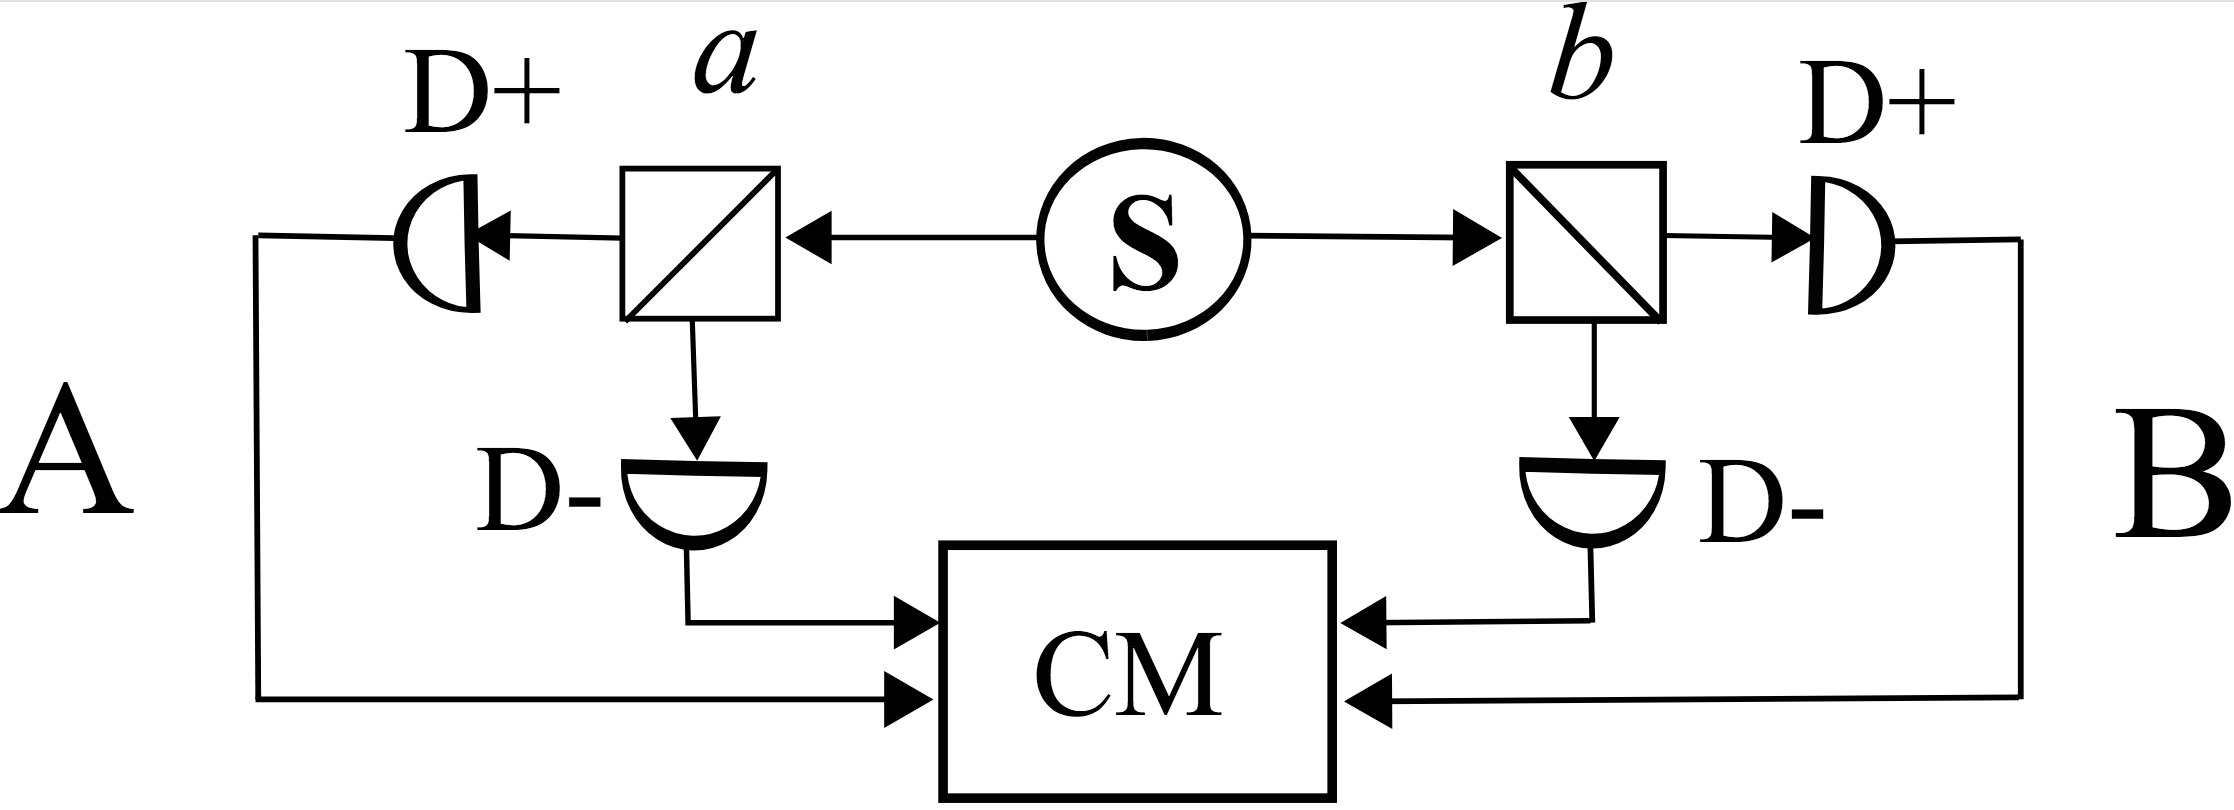
\includegraphics[width=0.6\textwidth, trim = 0 0 0 0]{./Bilder/Bell.png}
\caption{\label{fig_Bell}%
Experimenteller Aufbau eines Experiments zum Nachweis der Verletzung
der CHSH-Ungleichung: Eine Quelle (S) erzeugt zwei Photonen, die zu
\glq Alice\grq\ (A) bzw.\ \glq Bob\grq\ (B) geschickt werden.
Dort treffen die Photonen auf Polarisationsstrahlteiler ($a$ bzw.\ $b$) und werden
in Richtung der Detektoren (${\rm D}^+$ und ${\rm D}^-$) abgelenkt. 
Ein Koinzidenzmessger\"at (CM) registriert die eintreffenden Signale. Die beiden
Polarisationsstrahlteiler sind um die Strahlachse drehbar und lassen sich in jeweils
zwei verschiedene Positionen einstellen.}
\end{figure}

Seien $N^{++}, N^{+-}, N^{-+},N^{--}$ die H\"aufigkeiten, 
mit denen bei gegebener Winkel\-einstellung
der Filter die jeweiligen Detektoren reagiert haben ($+$ bedeutet
einen Teilchennachweis in Detektor $D^+$, $-$ einen Nachweis
in Detektor $D^-$; vgl.\ Abb.\ \ref{fig_Bell}), dann ist der zugeh\"orige Erwartungswert
f\"ur das Produkt der beiden Werte:
\begin{equation}
       E = \frac{(+1)N^{++} + (+1)N^{--} + (-1) N^{+-} + (-1) N^{-+}}{N^{++} + 
              N^{--} + N^{+-} + N^{-+}}
\end{equation}
F\"ur einen
total antikorrelierten verschr\"ankten EPR-Zustand
sind die Erwartungswerte f\"ur eine Winkeldifferenz
$\Delta \alpha$ in diesem Fall:
\begin{equation}
     E(\Delta \alpha) 
     = \frac{ \sin^2 \Delta \alpha + \sin^2 \Delta \alpha - \cos^2 \Delta \alpha - \cos^2 \Delta \alpha}{ \sin^2 \Delta \alpha + \sin^2 \Delta \alpha + \cos^2 \Delta \alpha + \cos^2 \Delta \alpha} = 
     \sin^2 \Delta \alpha - \cos^2 \Delta \alpha
          = - \cos 2 \Delta \alpha
\end{equation}
$\sin^2 \Delta \alpha$ ist die Wahrscheinlichkeit, dass die
beiden Teilchen denselben Messwert liefern (beide $+$ oder
beide $-$) und $\cos^2 \Delta \alpha$ ist die Wahrscheinlichkeit,
dass sie verschiedene Werte liefern ($+-$ bzw.\ $-+$).

F\"ur die Winkel $a=0^\circ$, $a'=45^\circ$, $b=22,5^\circ$ und 
$b'=67,5^\circ$ gibt es letztendlich f\"ur $\Delta \alpha$ nur
zwei Kombinationen: $(a,b') \rightarrow \Delta \alpha = 67,5^\circ$
und $(a,b), (a',b), (a',b') \rightarrow \Delta \alpha = \pm 22,5^\circ$.
Damit folgt schlie\ss lich:
\begin{equation}    
    E(S) = \cos (2\cdot 67,5^\circ) - 3 \cdot \cos ( 2\cdot 22,5^\circ) =
      - \frac{4}{\sqrt{2}} = - 2 \sqrt{2} \approx - 2,828   
\end{equation}  
Dieses\index{Quantum bound} 
Ergebnis liegt also um einen Faktor $\sqrt{2}$ au\ss erhalb
des Bereichs, der nach der CHSH-Ungleichung erlaubt w\"are
(man bezeichnet $2\sqrt{2}$ manchmal auch als \glqq quantum bound\grqq).
Das erscheint im ersten Augenblick zwar viel, doch da sich
jede Unsicherheit, beispielsweise bei der Ansprechgenauigkeit
der Detektoren, zu Ungunsten des Ergebnisses auswirkt,
war der experimentelle Nachweis der Verletzung nicht einfach.

In die CHSH-Ungleichung gehen nur zwei der drei in Abschnitt
\ref{sec_Espagnat} genannten Annahmen ein. Die kontrafaktische Implikation
ist\index{kontrafaktische Implikation} 
nicht erforderlich, da die Korrelation oder Antikorrelation
bez\"uglich derselben Orientierungen nicht vorausgesetzt
wurde. Allerdings kann die Ungleichung nur an einem
verschr\"ankten Zustand verletzt werden.

\subsection{Zusammenfassung}

Fassen wir das Ergebnis nochmals zusammen: Die Annahme, dass die
Messergebnisse schon vor der Messung festliegen, f\"uhrt auf de CHSH-Ungleichung.
Diese ist in der Quantentheorie verletzt, sodass diese Annahme nicht g\"ultig
ist. Die Ergebnisse entstehen also erst im Augenblick der Messung, allerdings
nicht willk\"urlich und an beiden Teilsystemen unabh\"angig, da in diesem Fall
die CHSH-Ungleichung erf\"ullt sein m\"usste. Man kommt also nicht umhin,
in der Quantentheorie eine Form von Nicht-Lokalit\"at zu fordern; anders lassen sich
die Ergebnisse nicht erkl\"aren. Diese Nicht-Lokalit\"at ist allerdings nicht
direkt beobachtbar, da die Korrelationen nicht zur gezielten \"Ubertragung von
Signalen genutzt werden k\"onnen. Gibt man die Lokalit\"at auf, lassen sich
zwar kausale Modelle konstruieren, welche die Verletzung der CHSH-Ungleichung
beschreiben, allerdings entstehen die Eigenschaften, die den Messergebnissen  
entsprechen, erst im Augenblick der Messung. Sie sind nicht vorherbestimmt.

Wie bei allen No-Go-Theoremen in der Physik ist es auch hier schwierig, genau
alle Annahmen aufzuz\"ahlen, die man als selbstverst\"andlich in die Schlussfolgerungen
gesteckt hat. Es wurde schon der sogenannte Superdeterminismus erw\"ahnt,
manchmal spricht man auch von \glqq no conspiracy\glqq\ oder vom \glqq freien Willen\grqq\
der Experimentierenden, die Einstellungen ($a$ oder $a'$ im einen Fall und $b$ oder $b'$
im anderen Fall) zu w\"ahlen. Alle Annahmen beziehen sich darauf, dass zwischen 
den Entscheidungen, welche beiden Observablen an einem konkreten Teilchenpaar
gemessen werden, und den verborgenen Parametern dieses Teilchenpaars, keine
Beziehungen bestehen: Die Ensembles, an denen zwei Observable gemessen werden,
sind bez\"uglich der Verteilung ihrer verborgenen Variablen gleich. 
 
Eine zweite Annahme betrifft die Struktur der Raumzeit. Sollte es bei verschr\"ankten
Systemen eine Art Wurmloch in der Raumzeit geben, d.h., auch wenn die Teilsysteme
f\"ur uns weit voneinander entfernt scheinen, sind sie doch noch unmittelbar zusammen,
kann die Nicht-Lokalit\"at umgangen werden. Weitere Annahmen beziehen sich auf
die Natur des \glqq Zustands\grqq. Sofern damit lediglich das Wissen einer Person gemeint
ist (und dieses Wissen breitet sich bestenfalls mit Lichtgeschwindigkeit aus), kann man
das Paradoxe umgehen. Allerdings erhebt sich dann die Frage, ob es \"uberhaupt
eine Realit\"at unabh\"angig von unserer Wahrnehmung gibt. 
%Einige dieser Fragen werden in Kap.\ \ref{chap_Interpretationen} nochmals aufgegriffen. 

\section*{Anmerkungen}
\subsection*{Die Richtungsunabh\"angigkeit des EPR-Zustands (Herleitung 1)}
\label{sec_EPR_A}

Eine allgemeine unit\"are Transformation in einem 2-dimensionalen komplexen
Vektorraum hat die Form
\begin{equation}
             U = \left( \begin{array}{cc} a & b \\ - b^* & a^* \end{array} \right)
             \hspace{1cm} {\rm mit} \hspace{0.6cm}  a a^* + b b^* = 1 \, . 
\end{equation}
Auf eine beliebige Basis $\{ |\pmb{e}_1 \rangle, |\pmb{e}_2\rangle$ wirkt diese Transformation
in der Form:
\begin{equation}
    | \pmb{f}_1 = a | \pmb{e}_1 \rangle + b |\pmb{e}_2 \rangle \hspace{0.5cm} , \hspace{0.5cm}
     | \pmb{f}_2 = -b^* | \pmb{e}_1\rangle + a^* |\pmb{e}_2 \rangle \, . 
\end{equation}
F\"ur den EPR-Zustand (ausgedr\"uckt in der $\pmb{f}$-Basis) folgt:
\begin{eqnarray}
    \frac{1}{\sqrt{2}} \big(  | \pmb{f}_1 \rangle \otimes | \pmb{f}_2 \rangle - 
        | \pmb{f}_2 \rangle \otimes | \pmb{f}_1 \rangle \big)  & = & \\ 
        & &  \hspace*{-5cm} =
    \frac{1}{\sqrt{2}} \Big(  \big( a | \pmb{e}_1 \rangle + b |\pmb{e}_2 \rangle \big) 
        \otimes  \big(  -b^* | \pmb{e}_1\rangle + a^* |\pmb{e}_2 \rangle \big)
         -  \big( -b^* | \pmb{e}_1\rangle + a^* |\pmb{e}_2 \rangle \big) 
            \otimes \big(  a | \pmb{e}_1 \rangle + b |\pmb{e}_2 \rangle \big)  \Big)       \\   
        & &  \hspace*{-5cm} =
  \frac{1}{\sqrt{2}} ( a a^* + b b^*) \big( | \pmb{e}_1 \rangle \otimes | \pmb{e}_2 \rangle - 
        | \pmb{e}_2 \rangle \otimes | \pmb{e}_1 \rangle \big)  \\
                & &  \hspace*{-5cm} =
  \frac{1}{\sqrt{2}} \big( | \pmb{e}_1 \rangle \otimes | \pmb{e}_2 \rangle - 
        | \pmb{e}_2 \rangle \otimes | \pmb{e}_1 \rangle \big)  
\end{eqnarray}

\subsection*{Die Teilspur zum EPR-Zustand (Herleitung 2)}
\label{sec_EPR_B}

Der Projektionsoperator zum EPR-Zustand (in einer Basis $\{ |\pmb{e}_i\rangle\}$)
ist
\begin{equation}
    P_{\rm EPR} =  \frac{1}{2} 
        \big( | \pmb{e}_1 \rangle_1 \otimes | \pmb{e}_2 \rangle_2 - 
        | \pmb{e}_2 \rangle_1 \otimes | \pmb{e}_1 \rangle_2 \big) 
         \big( {}_2\langle \pmb{e}_2 | \otimes {}_1\langle \pmb{e}_1 | - 
        {}_2\langle \pmb{e}_1 | \otimes {}_1\langle \pmb{e}_2 | \big) \,
\end{equation}
wobei hier der \"Ubersichtlichkeit halber die Vektoren noch mit einem
Index versehen sind, der anzeigt, ob der Vektor sich auf Hilbert-Raum 1 oder
2 bezieht. Bilden wir nun die Teilspur zu Hilber-Raum 2 und nutzen die
Orthogonalit\"at der Basisvektoren aus, 
$ {}_2 \langle \pmb{e}_i | \pmb{e}_j \rangle_2 = \delta_{ij}$, 
erhalten wir:
\begin{eqnarray}
   {\rm Sp}_2 P_{\rm EPR} 
    &=& \sum_{i=1}^2  {}_2\langle \pmb{e}_i | P_{\rm EPR} | \pmb{e}_i \rangle_2  \\
    &=&  \frac{1}{2}  \sum_{i=1}^2 {}_2\langle \pmb{e}_i |
        \big( | \pmb{e}_1 \rangle_1 \otimes | \pmb{e}_2 \rangle_2 - 
        | \pmb{e}_2 \rangle_1 \otimes | \pmb{e}_1 \rangle_2 \big) 
         \big( {}_2\langle \pmb{e}_2 | \otimes {}_1\langle \pmb{e}_1 | - 
        {}_2\langle \pmb{e}_1 | \otimes {}_1\langle \pmb{e}_2 | \big) |\pmb{e}_i \rangle_2  \\
     &=&   \frac{1}{2}    
     \big( | \pmb{e}_1 \rangle_1 {}_1 \langle \pmb{e}_1 | + | \pmb{e}_2 \rangle_1 {}_1 \langle \pmb{e}_2 | \big)
      = \frac{1}{2} \identity_1 \, .
\end{eqnarray}
Das gleiche Ergebnis erhalten wir, wenn wir den Erwartungswert von einer
beliebigen Observablen im Hilbert-Raum 1 betrachten, also von $A \otimes \identity_2$:
\begin{equation}
    {\rm Sp} P_{\rm EPR} (A \otimes \identity_2) 
    = \frac{1}{2} \big( {}_1 \langle \pmb{e}_1 | A | \pmb{e}_1 \rangle_1 +  
                {}_1 \langle \pmb{e}_2 | A | \pmb{e}_2 \rangle_1 \big)  =  \frac{1}{2} {\rm Sp}_1 A\, \identity_1 \, . 
\end{equation}


\begin{thebibliography}{99}
\bibitem{Aspect} Aspect, A., Grangier, Ph., Roger, G.; 
       {Experimental Realization of Einstein-Podolsky-Rosen-Bohm 
        Gedankenexperiment: A New Violation of Bell's Inequalities}; 
        Phys.\ Rev.\ Lett.\ 49 (1982) 91--94. \\
        Aspect, A., Dalibard, J., Roger, G.; {Experimental Test 
        of Bell's Inequalities Using Time-Varying Analyzers}; 
        Phys.\ Rev.\ Lett.\ 49 (1982) 1804--1807.
\bibitem{Bell} Bell, J.S.;  {\em Speakable and Unspeakable in 
        Quantum Physics}, 2.\ edition, Cambridge University Press (2004).                 
\bibitem{Bell4} Bell, J.S.; {\em On the Einstein-Podolsky-Rosen paradox};
        Physics 1 (1964) 195. Abgedruckt in \cite{Bell}.          
\bibitem{Bell3} Bell, J.S.; {\em On the problem of hidden variables
        in quantum theory}; Rev.\ Mod.\ Phys.~38 (1966) 447.
        Abgedruck in \cite{Bell}.
\bibitem{Bohr2} Bohr, N.; {\em Can quantum-mechanical description
        of physical reality be considered complete?}; Phys.\ Rev.\ 48
        (1935) 696.       
\bibitem{CHSH} Clauser, J.\,F., Horne, M.\,A., Shimony, A., Holt, R.\,A.;
      {\em Proposed experiment to test local hidden-variable theories}, 
      Phys.\ Rev.\ Lett.\ {\bf 23} (1969) 880-884.          
\bibitem{EPR} Einstein, A., Podolski, B., Rosen,
       N.; {\em Can quantum-mechanical description of
        physical reality be considered complete?}; Phys.\ Rev.\ 47
        (1935) 777--780.   
\bibitem{Espagnat} D'Espagnat, B.; {\em Quantentheorie und Realit\"at};
        Spektrum der Wissenschaft 1 (1980) 69. 
\bibitem{Gilder} Gilder, L.; {\em The Age of Entanglement:
         When Quantum Physics was Reborn}; Penguin Vintage (2009).
\bibitem{Heisenb} Heisenberg, W.; Anmerkungen im Anschluss des Artikels:
       Renninger, M.;  {\em Messung ohne St\"orung des Me\ss objekts}; Z.\ Physik 158 (1960) 417.
\bibitem{Neumann} von Neumann, J.; {\em Mathematische
    Grundlagen der Quantentheorie}; Springer (1932).       
\bibitem{Pauli} Pauli, W., Brief an Heisenberg vom 15.\ Juni 1935, in
             {\em Wolfgang Pauli - Scientific Correspondence with
             Bohr, Einstein, Heisenberg a.o.}, Karl von Meyenn (Hrsg.),
             Band II 1930--1939, Springer (1985).
\bibitem{Schroedinger} Schr\"odinger, E.; {\em Die gegenw\"artige
        Situation in der Quantenmechanik}; Die Naturwissenschaften 23
        (1935) 807--812, 823--828,  844-849.      
\bibitem{Yin} Yin, J., et al.; \textit{Satellite-based entanglement distribution over
      1200 kilometers}; Science 356 (2017) 1140.    
\end{thebibliography}


%\end{document}

